\documentclass[11pt]{article}

\usepackage[margin=1in]{geometry}
\usepackage{amsmath, amssymb}
\usepackage{siunitx}
\usepackage{graphicx}
\usepackage{hyperref}
\usepackage{tikz}
\usepackage{pgfplots}
\usepackage{enumitem}
\usepackage{parskip}
\usepackage{booktabs}
\usepackage{float}

\pgfplotsset{compat=1.18}

\title{APMA 2822B Homework 3 Report}
\author{Yash Agrawal}
\date{\today}

\begin{document}
\maketitle

\section*{Math Setup}

Most of the math setup for this assignment is identical to homework 3, except we use \(\sin^2\) instead of \(\sin \cdot \cos\) in our \(f(x, y)\) function. The final update equation is as follows:
\[
u[i, j] = \frac{1}{4} \left( u[i-1, j] + u[i+1, j] + u[i, j-1] + u[i, j+1] + 8\pi^2 h^2 \sin^2(2\pi x) \right)
\]

\section*{Results}

I implemented two new kernels for this assignment. The first uses shared memory and a single GPU to accelerate both the update and residual loops. The second uses MPI and distributed memory to use multiple GPUs to accelerate both loops. This version used 8 processes, and shared 4 GPUs. 

The results are summarized below, where N is the length of one side of the array (the array is size \(N \times N\)). Copy here represents the time taken to move the residual values from the GPU to the CPU for convergence checking.

\begin{table}[h]
    \centering
    \begin{tabular}{@{} l r r r r r r r @{}}
        \hline
        Kernel & N & Time (s) & BW (GB/s) & Alloc (ms) & Residual (s) & Update (s) & Copy (s) \\
        \hline
        Shared 
        & 256 & 2.41 & 40.46 & 115.97 & 0.51 & 0.48 & 0.51 \\
        & 512 & 10.057 & 202.36 & 115.11 & 2.57 & 2.62 & 2.020 \\
        & 1024 & 59.28 & 422.99 & 122.01 & 16.85 & 22.65 & 6.95 \\
        & 2048 & 319.226 & 1257.92 & 0.26 & 58.21 & 88.37 & 31.72 \\
        \hline
        Distributed 
        & 256 & 3.79 & 25.67 & 0.10 & 0.49 & 0.43 & 0.50 \\
        & 512 & 14.53 & 107.62 & 0.11 & 2.13 & 1.94 & 1.88 \\
        & 1024 & 61.67 & 406.61 & 0.18 & 9.47 & 10.19 & 8.37 \\
        & 2048 & 567.51 & 707.57 & 117.36 & 181.02 & 277.37 & 44.83 \\
        \hline
    \end{tabular}
\end{table}

Additionally, both kernels produce identical, correct results in the exact same number of iterations as the CPU implementation (with the updated equation) from homework 3 (37,144 for N=256,149,170 for N=512, 597,860 for N=1024, 2,393,789 for N=2048). The CPU implementation, however, did not complete for N=2048.

\section*{Analysis}

We find that, as expected, GPU acceleration significantly improves our performance. We also find that the improvement is more significant for larger arrays. On arrays of size \(1024 \times 1024\), GPU acceleration provides around a 4x speedup over the CPU OpenMP implementation from homework 3 (which was the fastest CPU implementation). Additionally, on arrays of size \(2048 \times 2048\), GPU acceleration sped up the solution enough to converge.

For small arrays the distributed kernel is slower than the shared kernel, likely due to the overhead of MPI communication and the kernels themselves being much too fast for any speed increase caused by each kernel operating on smaller subarrays to offset this overhead. However, as the array size increases, the distributed kernel starts to outperform the shared kernel. This is likely because the distributed kernel is able to utilize multiple GPUs, which provides more total memory bandwidth and compute power than a single GPU.

\section*{Roofline Model}

The derivation for the roofline model of the update loop as well as the residual loop is identical to homework 3. I have included that roofline model here as well, with the performance of the hardware modified to reflect GPU specs.

\begin{figure}[H]
    \centering
    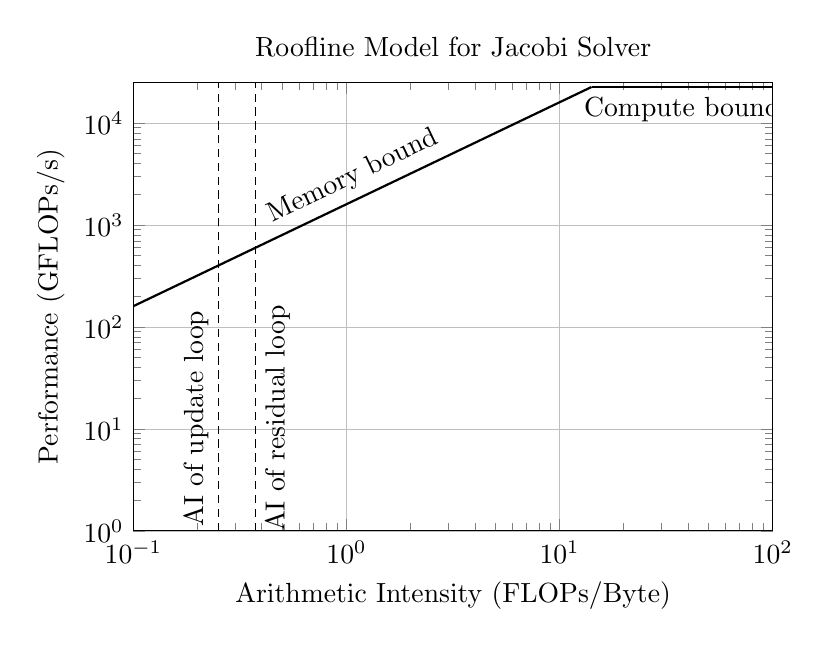
\begin{tikzpicture}
        \begin{axis}[
            title={Roofline Model for Jacobi Solver},
            xlabel={Arithmetic Intensity (FLOPs/Byte)},
            ylabel={Performance (GFLOPs/s)},
            xmode=log,
            ymode=log,
            xmin=0.1, xmax=100,
            ymin=1, ymax=25000,
            grid=major,
            major grid style={line width=.2pt,draw=gray!50},
            width=0.8\linewidth,
            height=0.6\linewidth,
        ]

        % Parameters
        \def\bandwidth{1600} % Memory bandwidth in GB/s
        \def\compute{22600}  % Peak performance in GFLOPs/s
        \def\cpuai{\compute/\bandwidth} % CPU arithmetic intensity

        % Memory bound line
        \addplot [thick, domain=0.1:{\cpuai}] {\bandwidth * x}
            node[pos=0.5, above, sloped] {Memory bound};

        % Compute bound line
        \addplot [thick, domain={\cpuai}:100] {\compute}
            node[pos=0.5, below] {Compute bound};

        % Operation points
        \addplot[densely dashed] coordinates {(0.25,1) (0.25,25000)}
            node[pos=0.25, sloped, above] {AI of update loop};

        \addplot[densely dashed] coordinates {(0.375,1) (0.375,25000)}
            node[pos=0.25, sloped, below] {AI of residual loop};

        \end{axis}
    \end{tikzpicture}
\end{figure}

\end{document}